\section{Results}
\label{sec:Results}

In this section, we present the results obtained in the two variants of the \ApproachName{} approach (with the simulation-based and the test-based objective functions) and the PCG baseline in \CaseStudy{}.

\subsection{Research Question 1}

Table~\ref{tab:results} shows the mean values and standard deviations for Q$_{DURATION}$ for each variant and baseline. Both variants (I$_S$ and I$_T$) obtained better results than the baseline (Base). Specifically, I$_S$ (simulations as objective function) yielded the best results, followed by I$_T$ (tests as objective function) and then baseline.

\begin{table*}[ht!]
\centering
\caption{Mean values and standard deviations for Q$_{DURATION}$ for each variant.}
\label{tab:results}
\begin{tabular}{@{}ccccccc@{}}
\toprule
                                   & \multicolumn{6}{c}{\ApproachName{} with simulation-based variant (I$_S$)}                                           \\ \cmidrule(l){2-7} 
                                   & Argos            & Maia              & Orion            & Teuthus           & Vermis            & Overall           \\ \midrule
                                   \rowcolor[HTML]{C0C0C0}
\multicolumn{1}{r}{\cellcolor[HTML]{FFFFFF}{Q$_{DURATION}$}} & 43.92 $\pm$ 9.30 & 43.08 $\pm$ 12.09 & 48.86 $\pm$ 8.69 & 60.78 $\pm$ 7.38  & 69.90 $\pm$ 10.52 & 53.31 $\pm$ 14.26 \\ \midrule
                                   & \multicolumn{6}{c}{\ApproachName{} with test-based variant (I$_T$)}                                                 \\ \cmidrule(l){2-7} 
                                   & Argos            & Maia              & Orion            & Teuthus           & Vermis            & Overall           \\ \midrule
\multicolumn{1}{r}{Q$_{DURATION}$} & 32.17 $\pm$ 6.94 & 29.52 $\pm$ 9.34  & 31.41 $\pm$ 6.83 & 46.33 $\pm$ 10.54 & 42.50 $\pm$ 12.96 & 36.39 $\pm$ 11.72 \\ \midrule
                                   & \multicolumn{6}{c}{PCG Baseline (Base)}                                                                             \\ \cmidrule(l){2-7} 
                                   & Argos            & Maia              & Orion            & Teuthus           & Vermis            & Overall           \\ \midrule
\multicolumn{1}{r}{Q$_{DURATION}$} & 20.15 $\pm$ 1.86 & 8.43 $\pm$ 1.81   & 32.97 $\pm$ 0.85 & 19.53 $\pm$ 1.88  & 25.48 $\pm$ 3.31  & 21.31 $\pm$ 8.32  \\ \bottomrule
\end{tabular}
\end{table*}

Figure~\ref{fig:results} shows the results of the evaluation execution of our approach when using the two objective functions (simulation-Based and test-Based) from \ApproachName{} and the Baseline. The executions are grouped by each host (boss of \CaseStudy{}) that has been used in our experiment (Argos, Maia, Orion, Teuthus, and Vermis). The last column, with shaded background, shows the average of all the hosts for each objective function and the baseline. 
%In addition, the oracle indicates the value obtained by the human-generated final boss models that were obtained from \CaseStudy{}.

Each boxplot is generated from the results of each host obtained from the transplantation of (\ApproachName{}) or generation (baseline). Each boxplot represents 645 values of a specific host-organ transplantation (\ApproachName{}) or 645 generations from a specific host (baseline). Each value in the boxplot is the mean value (between the 30 independent runs) of the quality indicator (Q$_{DURATION}$) for one of the transplants (\ApproachName{}) or generations (baseline).

%Figure~\ref{fig:results} shows in each column how the quality values obtained for each of the three strategies studied in our evaluation differ from the values for the models generated by the developers, which are represented by the horizontal red dashed lines that cross each host column. The boxplots that are closer to the horizontal lines are more similar in quality to the models produced by the developers. Additionally, the use of boxplots allows for the representation of the different results for the strategies used.

\textbf{RQ$_1$ answer. }
The variants obtained an average value of 44.85\% in Q$_{DURATION}$, with I$_S$ being the variant that obtained the best results overall (53.31\% in Q$_{DURATION}$). I$_T$ obtained 36.39\% in the overall Q$_{DURATION}$, which also outperformed the baseline. The baseline obtained the worst Q$_{DURATION}$. All in all, the results reveal that leveraging simulations as objective function pays off in the context of PCT, yielding 1.5x better results than test-based variant and 2.5x better results than baseline.

\subsection{Research Question 2}

To properly compare the approaches, all of the data resulting from the empirical analysis was analyzed using statistical methods following the guidelines in~\cite{Arcuri2014}.

The analysis that we must follow depends on the properties of the data. Since our data does not follow a normal distribution in general, our analysis requires the use of non-parametric techniques. There are several tests for analyzing this kind of data; however, the Quade test has shown that it is more powerful than the others when working with real data~\cite{Garcia2010}. In addition, according to Conover~\cite{Conover1999}, the Quade test has shown better results than the others when the number of algorithms is low (no more than four or five algorithms).

The $p-Values$ obtained are lower than $2.2x10^{-16}$ for Q$_{DURATION}$. Since the $p-Values$ are smaller than 0.05, we can state that there are differences among the algorithms for the quality indicator of Q$_{DURATION}$.

\begin{table}[H]
\centering
\caption{Holm's post hoc $p-Values$ for each pair-wise comparison.}
\label{tab:postHoc}
\begin{tabular}{@{}rc@{}}
\toprule
               & Q$_{DURATION}$ \\ \midrule
I$_S$ vs Base  & $<2x10^{-16}$  \\
I$_S$ vs I$_T$ & $<2x10^{-16}$  \\
I$_T$ vs Base  & $<2x10^{-16}$  \\ \bottomrule
\end{tabular}
\end{table}

However, with the Quade test, we cannot know which of the algorithms gives the best performance. In this case, the performance of each algorithm should be individually compared against all of the other alternatives. In order to do this, we perform an additional post hoc analysis. This kind of analysis performs a pair-wise comparison among the results of each algorithm, determining whether statistically significant differences exist among the results of a specific pair of algorithms.

Table~\ref{tab:postHoc} shows the $p-Values$ of the Holm's post hoc analysis for each pair-wise comparison and quality indicator. All of the $p-Values$ obtained in Q$_{DURATION}$ were smaller than their corresponding significance threshold value ($0.05$), indicating that the differences in solution quality between the two variants and the baseline are significant.

\textbf{RQ$_2$ answer. }
Since the Holm's post hoc $p-Values$ for Q$_{DURATION}$ that are shown in Table~\ref{tab:postHoc} are smaller than $0.05$, we can state that there are significant differences between the variants and the baseline.

\subsection{Research Question 3}

When comparing algorithms with a large enough number of runs, statistically significant differences can be obtained even if they are so small as to be of no practical value~\cite{Arcuri2014}. Thus, it is important to assess if an algorithm is statistically better than another and to assess the magnitude of the improvement. Effect size measures are needed to analyze this.

\begin{table}[H]
\centering
\caption{Effect size measures for comparing each pair of algorithms in \CaseStudy{}.}
\label{tab:effectSize}
\begin{tabular}{@{}rc@{}}
\toprule
               & Â$_{12}$          \\ \cmidrule(l){2-2} 
               & Q$_{DURATION}$    \\ \midrule
I$_S$ vs Base  & 0.0121531         \\
I$_S$ vs I$_T$ & 0.1712710         \\
I$_T$ vs Base  & 0.1411910         \\ \midrule
               & Cliff's Delta     \\ \cmidrule(l){2-2} 
               & Q$_{DURATION}$    \\ \midrule
I$_S$ vs Base  & 0.9756914 (large) \\
I$_S$ vs I$_T$ & 0.6574437 (large) \\
I$_T$ vs Base  & 0.7175939 (large) \\ \bottomrule
\end{tabular}
\end{table}

For a non-parametric effect size measure, we use Vargha and Delaney's $\hat{A}_{12}$~\cite{Vargha2000,Grissom2005}. $\hat{A}_{12}$ measures the probability that running one algorithm yields higher values than running another algorithm. If the two algorithms are equivalent, then $\hat{A}_{12}$ will be 0.5.

Table~\ref{tab:effectSize} shows the values of the effect size statistics between pair-wise comparisons of algorithms in \CaseStudy{}. Specifically, the upper part of the table shows the $\hat{A}_{12}$ values, whereas the lower part of the table shows Cliff's Delta~\cite{Cliff1996} values for Q$_{DURATION}$. From the results, we can determine that the performance results obtained by \ApproachName{} with the simulation-based variant, \ApproachName{} with the test-based variant, and the PCG baseline are significant in Q$_{DURATION}$. The magnitude of improvement using \ApproachName{} instead of the baseline can be interpreted as being large based on the magnitude scales~\cite{Romano2006} of the Cliff's Delta values. Hence, \ApproachName{} has an actual impact on performance. The highest differences between \ApproachName{} and the baseline are obtained when the simulation-based variant is used, obtaining better results in Q$_{DURATION}$ for 97\% of the runs.

\textbf{RQ$_3$ answer. }
We can draw conclusions about how much the quality of the solution is influenced by each variant of \ApproachName{} compared to baseline from the results of Table~\ref{tab:effectSize}. The results reveal that the magnitude of improvement in Q$_{DURATION}$ using any variant is large compared to the baseline according to the magnitude scales~\cite{Romano2006} of the Cliff's Delta values.


\begin{figure*}[ht!]
    \centering
    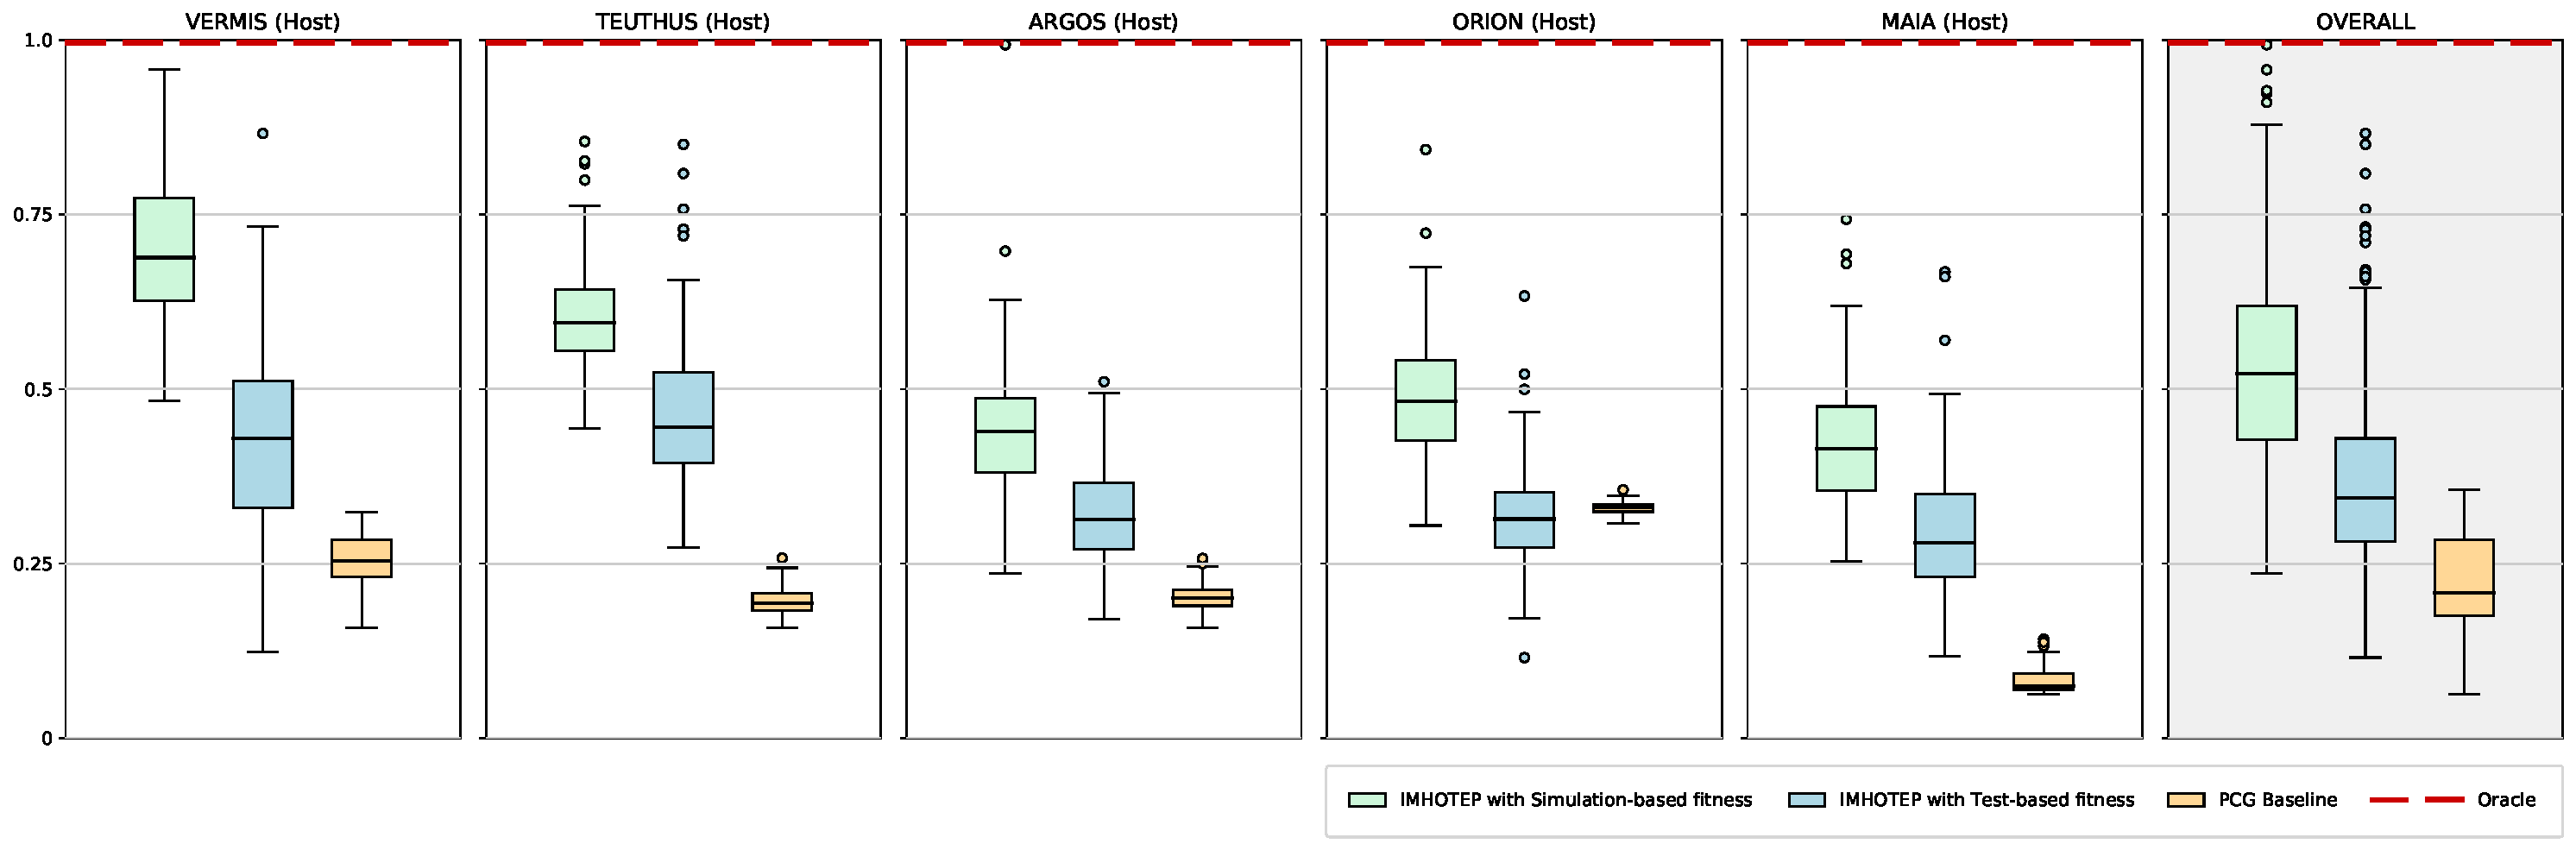
\includegraphics[width=\textwidth]{Figures/Imhotep_with_legend_and_oracle_average-v4.pdf}
    \caption{Results of our \ApproachName{} approaches (simulation-based and test-based) and the baseline for the quality measurement (Q$_{DURATION}$).}
    \label{fig:results}
\end{figure*}


% To have more detail about the results presented in Figure~\ref{fig:results} we include Table~\ref{tab:mean_sd} and Table~\ref{tab:max_min}. Table~\ref{tab:mean_sd} presents the results of our evaluation in terms of their mean values and their corresponding standard deviation. On other hand, Table~\ref{tab:max_min} shows the maximum and minimum values of the results. On both tables, we have the respective results of each host used in our experiment (Vermis, Teuthus, Argos, Orion, and Maia), and the last column shows the average of all the hosts.

% \textbf{RQ1 answer.} The results in Figure~\ref{fig:results} shows how simulation-based \ApproachName{} variant reaches the closer results to the oracle. Table~\ref{tab:max_min} shows that in two cases (Vermis and Maia) our approach is capable to obtain even better results than the oracle.

% \textbf{RQ2 answer.} Observing Table~\ref{tab:mean_sd} we can notice the difference in quality between our simulation-based and test-based variants. Simulation-based variant obtains 17\% better results than our test-based variant. 

% \textbf{RQ3 answer.} We can draw conclusions about the difference between \ApproachName{} and the baseline from the results of Table~\ref{tab:mean_sd}. The results reveal that simulation-based and test-based variants from our approach compared to the baseline obtain 32\% and 25\% respectively better results than the baseline. Table~\ref{tab:max_min} also reveals how there is a significant difference of 0.93 in the maximum values that simulation-based and the baseline can achieve, and 0.51 comparing test-based and the baseline.

% \begin{table*}[t!]
%     \caption{Mean Values and Standard Deviations}
%     \label{tab:mean_sd}
%     \centering
%     \resizebox{\textwidth}{!}{%
%     \begin{tabular}{llllllll}
%     \toprule
%     &\multicolumn{1}{c}{Vermis}
%     &\multicolumn{1}{c}{Teuthus}
%     &\multicolumn{1}{c}{Argos}
%     &\multicolumn{1}{c}{Orion}
%     &\multicolumn{1}{c}{Maia}
%     &\multicolumn{1}{c}{Overall}
%     \\ \midrule
%     Simulation
%     & 0.699 $\pm$ 0.105 & 0.607 $\pm$ 0.074 & 0.439 $\pm$ 0.093 & 0.488 $\pm$ 0.087 & 0.430 $\pm$ 0.121 & 0.533 $\pm$ 0.142       
%     \\
%     Test
%     & 0.424 $\pm$ 0.130 & 0.463 $\pm$ 0.105 & 0.321 $\pm$ 0.069 & 0.314 $\pm$ 0.068 & 0.295 $\pm$ 0.093 & 0.363 $\pm$ 0.117        
%     \\
%     Baseline
%     & 0.254 $\pm$ 0.033 & 0.195 $\pm$ 0.018 & 0.201 $\pm$ 0.018 & 0.329 $\pm$ 0.008 & 0.084 $\pm$ 0.018 & 0.213 $\pm$ 0.083
%     \\ \midrule     
% \end{tabular}
% }
% \end{table*}

% \begin{table*}[t!]
%     \caption{Max and Min values.}
%     \label{tab:max_min}
%     \centering
%     \resizebox{\textwidth}{!}{%
%     \begin{tabular}{lllllllllllll}
%     \toprule
%     & \multicolumn{2}{c}{Vermis}
%     & \multicolumn{2}{c}{Teuthus}
%     & \multicolumn{2}{c}{Argos}
%     & \multicolumn{2}{c}{Orion}
%     & \multicolumn{2}{c}{Maia}
%     & \multicolumn{2}{c}{Overall}
%     \\ \midrule
%     \multicolumn{1}{c}{} 
%     & \multicolumn{1}{c}{Max} & \multicolumn{1}{c}{Min} 
%     & \multicolumn{1}{c}{Max} & \multicolumn{1}{c}{Min} 
%     & \multicolumn{1}{c}{Max} & \multicolumn{1}{c}{Min}
%     & \multicolumn{1}{c}{Max} & \multicolumn{1}{c}{Min} 
%     & \multicolumn{1}{c}{Max} & \multicolumn{1}{c}{Min} 
%     & \multicolumn{1}{c}{Max} & \multicolumn{1}{c}{Min} 
%     \\
%     Simulation & 1.042 & 0.482   & 0.854 & 0.443   & 0.992 & 0.235   & 0.842 & 0.304   & 1.285 & 0.253   & 1.285 & 0.235                          
%     \\
%     Test & 0.866 & 0.123   & 0.850 & 0.273   & 0.510 & 0.170   & 0.633 & 0.115   & 0.667 & 0.117   & 0.866 & 0.115   
%     \\
%     Baseline & 0.323 & 0.157   & 0.257 & 0.158   & 0.257 & 0.157   & 0.355 & 0.307   & 0.141 & 0.063    & 0.355 & 0.063
%     \\ \midrule                     
% \end{tabular}
% }
% \end{table*}